% !TEX program = pdflatex
\documentclass[10pt]{article}
\usepackage[a3paper,landscape,left=7mm,right=7mm,top=10mm,bottom=10mm]{geometry}
\usepackage[T1]{fontenc}
\usepackage[utf8]{inputenc}
\usepackage{tgschola}
\usepackage{microtype}
\usepackage{amsmath,amssymb,mathtools,bm}
\usepackage{booktabs,array,tabularx}
\usepackage{enumitem}
\usepackage{xcolor}
\usepackage{tikz}
\usepackage[most]{tcolorbox}
\usepackage{graphicx}
\usepackage{adjustbox}
\usepackage{ragged2e}
\usepackage{hyperref}
\hypersetup{colorlinks=true,linkcolor=blue,urlcolor=blue}

% ---------- Visual system ----------
\definecolor{Accent}{HTML}{3478E5}
\definecolor{Ink}{HTML}{252B33}
\definecolor{Muted}{HTML}{68717D}
\definecolor{Rule}{HTML}{D7DCE2}
\definecolor{Pale}{HTML}{F1F6FF}
\definecolor{Soft}{HTML}{F7F8FA}
\definecolor{Good}{HTML}{2E7D5B}
\definecolor{Warm}{HTML}{A7641D}

\newcommand{\titlefont}{\bfseries}
\newcommand{\codefont}{\ttfamily}
\color{Ink}
\pagestyle{empty}
\setlength{\parindent}{0pt}
\setlength{\parskip}{2.5pt}
\setlist[itemize]{leftmargin=1.2em,itemsep=1.2pt,topsep=1.5pt}

% ---------- Reusable poster objects ----------
\newcommand{\blue}[1]{\textcolor{Accent}{#1}}
\newcommand{\postersection}[1]{%
  \vspace{1.2mm}\noindent{\raggedright\fontsize{17.5}{19.5}\selectfont\titlefont #1\par}
  \vspace{.6mm}\textcolor{Rule}{\rule{\linewidth}{0.6pt}}\vspace{.9mm}}
\newcommand{\postersubsection}[1]{%
  \vspace{.8mm}{\fontsize{13.2}{14.5}\selectfont\titlefont #1}\par\vspace{.3mm}}
\newcommand{\tinylabel}[1]{{\codefont\fontsize{7.5}{8.3}\selectfont\color{Muted} #1}}
\newcommand{\keyeq}[1]{\begin{tcolorbox}[enhanced,boxrule=.7pt,colframe=Ink,
  colback=white,arc=2.2mm,left=2.5mm,right=2.5mm,top=1.8mm,bottom=1.8mm]#1\end{tcolorbox}}

\newtcolorbox{infobox}[1][]{enhanced,breakable,boxrule=.7pt,colframe=Rule,
  colback=Soft,arc=2.2mm,left=2.5mm,right=2.5mm,top=1.8mm,bottom=1.8mm,#1}
\newtcolorbox{bluebox}[1][]{enhanced,breakable,boxrule=.9pt,colframe=Accent,
  colback=Pale,arc=2.2mm,left=2.5mm,right=2.5mm,top=1.8mm,bottom=1.8mm,#1}

% Preserve the central message as a reusable blue object.
\newcommand{\coreideabox}{%
\begin{bluebox}
\textbf{Core idea:}
\begin{enumerate}[leftmargin=1.5em,itemsep=.5mm,topsep=.6mm]
\item Checking the certificate conditions is much less expensive for ReLU
networks.
\item Because we can handle a piecewise quadratic network, we can compose
multiple certificates by taking their minimum.
\end{enumerate}
\end{bluebox}}

\newcommand{\statusdot}[1]{\tikz[baseline=-.55ex]\fill[#1] (0,0) circle (1.25mm);}

\begin{document}
\begin{adjustbox}{max totalsize={\textwidth}{\textheight},center}
\begin{minipage}{\textwidth}
\begin{minipage}[t]{\textwidth}
\centering
\resizebox{.97\textwidth}{!}{\titlefont It\^o--Tanaka Certificates: Towards Scalable SDE Certification through Compositionality}\par
\vspace{1.4mm}
{\fontsize{11.5}{13}\selectfont \blue{Filip Morawiec}\quad $\cdot$ \quad
University of Birmingham Summer Research Programme \quad $\cdot$ \quad 2026}\par
\vspace{.7mm}
{\fontsize{9.2}{10.5}\selectfont\color{Muted}
From exact reach--avoid guarantees to neural region discovery and local-time conditions by construction.}
\end{minipage}

\vspace{3mm}
\fontsize{9}{10.5}\selectfont
% ======================== FOUR READING COLUMNS ========================
\begin{minipage}[t]{0.235\textwidth}
\postersection{1. Introduction}
Consider the problem of ensuring that a continuous system behaves safely under
uncertainty---for example, that a humanoid robot does not fall over while
walking. One way to ensure safety is to perform many experiments. For such
complex systems, however, this is not feasible. Neural Continuous-Time
Supermartingale Certificates~[1] instead give exact probabilistic guarantees of
safety for stochastic differential equations (SDEs) of the form
\[
dX_t=f(X_t)\,dt+\sigma(X_t)\,dW_t,
\qquad X_t\in K\subset\mathbb R^d,
\]
over a compact domain $K\subset\mathbb R^d$.

\begin{center}
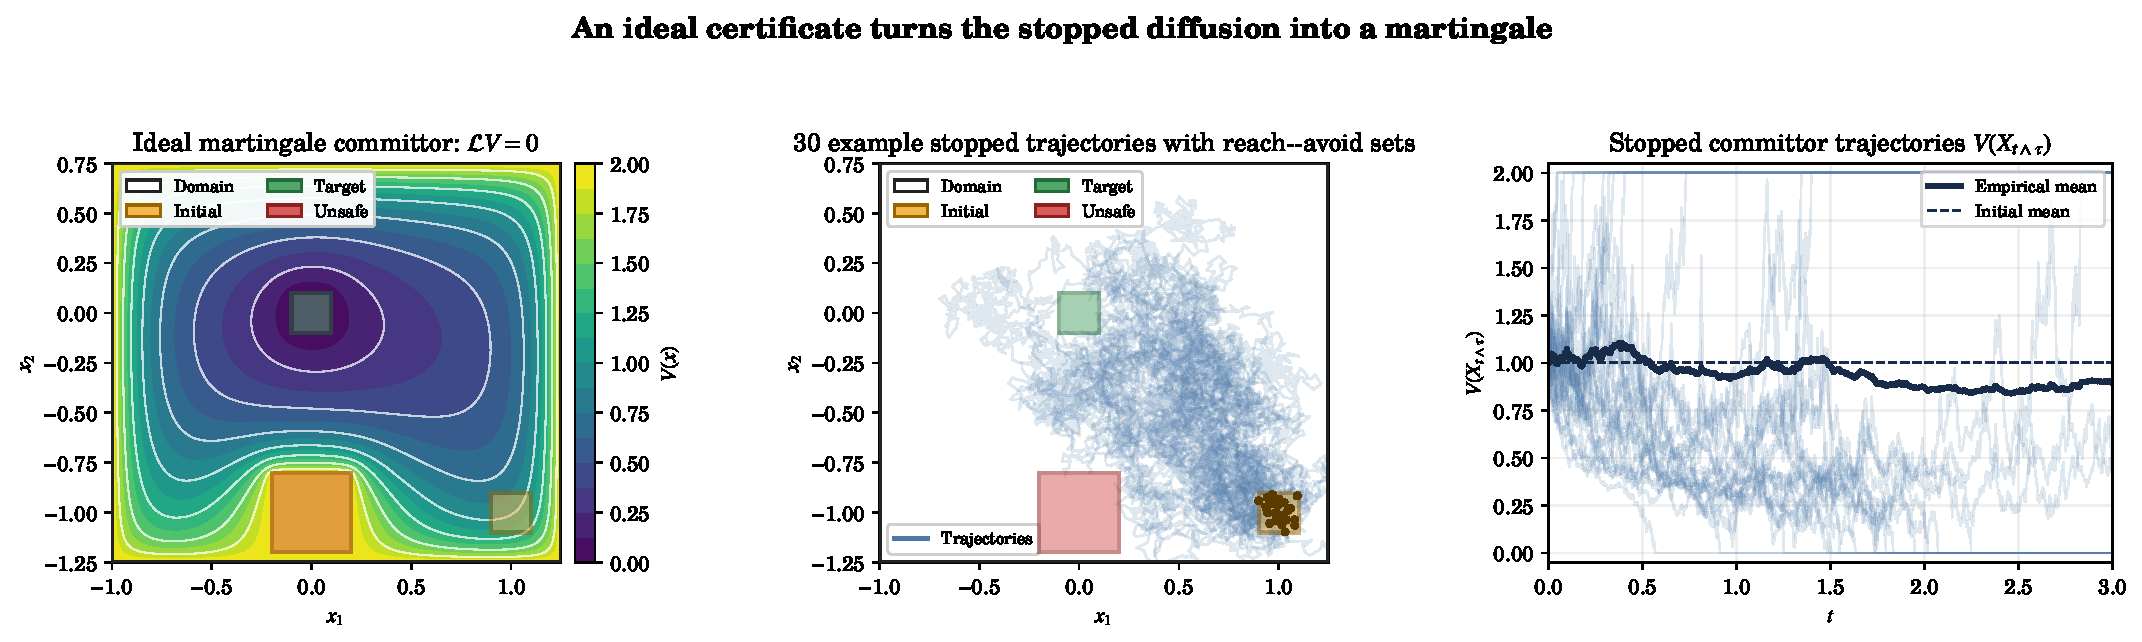
\includegraphics[width=\linewidth]{figures/intro_martingale_committor.pdf}
\end{center}

\postersubsection{Problem setup}
Given an initial set $X_0$, a target set $X_T$, an unsafe set $X_u$, and
$\alpha<\beta$, assume we find a nonnegative function $V:K\to\mathbb R$ such
that
\[
\sup_{X_0}V\leq\alpha<\beta,
\qquad
\inf_{X_u}V\geq\beta,
\qquad
\inf_{\partial K\setminus X_T}V\geq\beta.
\]
Stop on reaching $X_T$, $\partial K$, or the superlevel set $\{V\geq\beta\}$.

\keyeq{
\textbf{Theorem (reach--avoid guarantee).} If the stopped process
$V(X_{t\wedge\tau})$ is a supermartingale, then
\[
\mathbb P\!\left(\tau_{V\geq\beta}<
\tau_{\partial K}\wedge\tau_{X_T}\right)
\leq\frac{\alpha}{\beta}.
\]
Because $V\geq\beta$ on $X_u$, this bounds the probability of reaching the
unsafe set before the target without first leaving the certified domain.
}

\postersection{2. It\^o--Tanaka certificates}
In practice, we want to find $V$ using neural networks. To ensure that $V$ is a
supermartingale, we must check conditions relating $V$, $f$, and $\sigma$.
Suppose $V$ is continuous and twice differentiable inside polyhedral cells
$K_i$. Expanding the multidimensional It\^o--Tanaka formula separates the
drift, martingale, and interface-local-time effects:
\begin{align*}
V(X_{t\wedge\tau})={}&V(X_0)+\int_0^{t\wedge\tau}\mathcal LV(X_s)\,ds+M_t\\[-1mm]
&+\frac12\sum_F\int_0^{t\wedge\tau}\gamma_F(X_s)\,dL_s^F,
\end{align*}
where
\[
\mathcal LV=\nabla V^\top f+\tfrac12\operatorname{tr}(\sigma\sigma^\top\nabla^2V),
\quad
\gamma_F=(\nabla V_j-\nabla V_i)^\top n_{i\to j,F}.
\]

\begin{bluebox}
\textbf{Theorem (It\^o--Tanaka certificate).} If the generator condition
$\mathcal LV_i\leq0$ and the local-time condition $\gamma_F\leq0$
hold outside $X_T$ and below $\beta$, then---under the standard integrability
assumption---$V(X_{t\wedge\tau})$ is a supermartingale.
\end{bluebox}
\end{minipage}\hfill
% --------------------------------------------------------
\begin{minipage}[t]{0.235\textwidth}
\postersection{3. Piecewise-quadratic neural network}
We parameterize the certificate as
\[
V(x)=\sum_{k=1}^{m}\lambda_k\phi(z_k(x))+c,
\]
where
\[
z(x)=\texttt{NN}(x)
=W_L\operatorname{ReLU}\!\bigl(\cdots
\operatorname{ReLU}(W_1x+b_1)\cdots\bigr)+b_L
\]
and $\phi=\texttt{PiecewiseQuadratic1D}$ is a fixed continuous
piecewise-quadratic activation.

The hidden ReLU network partitions the input domain into polyhedral cells. On
each cell, $z(x)$ is affine; after refining by the pieces of $\phi$, the scalar
certificate has the exact form
\[
V_i(x)=c_i+p_i^\top x+\tfrac12x^\top Q_i x,
\qquad K_i=\{x:A_ix\leq b_i\}.
\]
Thus $\nabla V_i=p_i+Q_ix$ and $\nabla^2V_i=Q_i$ are explicit, making the
generator and interface conditions algebraic.

\begin{infobox}
\textbf{Why not a plain ReLU certificate?} A plain ReLU network is only
piecewise linear and has no curvature inside its cells. Consider
$dX_t=dt+\sqrt2\,dW_t$ on $[0,1]$, and require
$V(0)<V(1)$. For continuous piecewise-linear $V$, the local-time condition
makes the slopes nonincreasing. Yet increasing overall requires the first
linear piece to have slope $a_i>0$. Since $V''=0$ in its interior,
\[
\mathcal LV=V'+\tfrac12(2)V''=a_i>0,
\]
contradicting the generator condition. Kinks alone cannot repair this failure.

\begin{center}
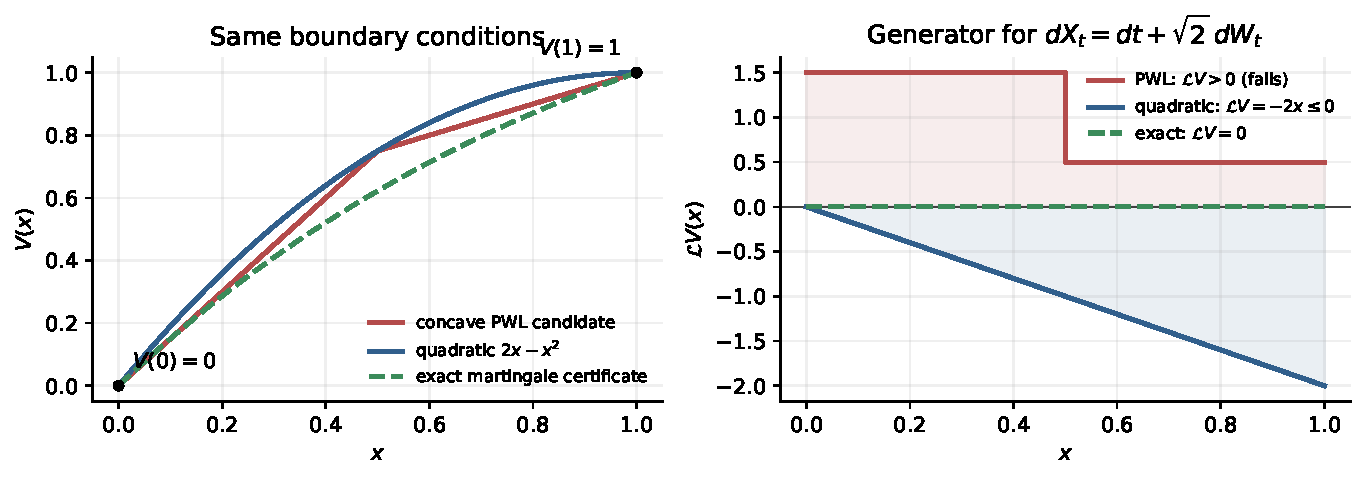
\includegraphics[width=.98\linewidth]{../log/figures/motivating_counterexample.pdf}
\end{center}

\textbf{Curvature repairs the failure.} The quadratic
$V(x)=2x-x^2$ has the same endpoint values, while
\[
\mathcal LV=(2-2x)+\tfrac12(2)(-2)=-2x\leq0.
\]
The negative curvature contribution compensates for the positive drift.
\end{infobox}

\coreideabox
\end{minipage}\hfill
% --------------------------------------------------------
\begin{minipage}[t]{0.235\textwidth}
\postersection{4. Pairwise-interface bottleneck}
Only adjacent full-dimensional regions sharing a facet contribute local time,
but discovering $N$ neural regions may already be exponential in depth and a
na\"ive pairwise search costs $O(N^2)$. The baseline verifier constructs the
actual adjacency graph, but the long-term goal is to avoid the facet check.

\postersubsection{Guarantee the sign by construction}
Split regular and singular curvature:
\[
\boxed{\qquad V_\theta(x)=S_\theta(x)-C_\psi(x).\qquad}
\]
$S_\theta$ is $C^1$ and piecewise quadratic, for example
\[
S_\theta(x)=c+p^\top x+\tfrac12x^\top Hx
+\tfrac12\sum_kv_k\operatorname{ReLU}(a_k^\top x+b_k)^2,
\]
while $C_\psi$ is convex and piecewise affine: either a ReLU input-convex neural
network or $\max_r(a_r^\top x+b_r)$.

\begin{bluebox}
The $C^1$ branch has no singular surface curvature. Convexity gives
\[
D^2_{\mathrm{sing}}V_\theta
=-D^2_{\mathrm{sing}}C_\psi\preceq0,
\]
so every local-time jump has the required sign \emph{without} discovering the
facet adjacency graph. Value bounds and the interior generator still require
verification.
\end{bluebox}

\postersubsection{Expressivity trade-off}
The construction controls only the nonsmooth curvature: $S_\theta$ may retain
indefinite ordinary curvature. However, global convexity of $C_\psi$ is stronger
than constraints only on reachable facets, and its CPWL gradient jumps are
piecewise constant rather than affine along a general PWQ facet.

\postersection{5. Current contribution}
\begin{itemize}
\item Exact multidimensional neural-cell discovery with PWQ coefficients.
\item A sound geometric 2D verifier for values, generator, continuity, and local-time jumps.
\item Residual ICNN and max-affine architectures with the jump sign built in.
\item A structural verifier that omits facet enumeration for these architectures.
\item A successfully trained and exactly verified construction-safe certificate, shown below.
\end{itemize}

\textcolor{Muted}{\fontsize{8.2}{9.3}\selectfont Exact verification currently
targets 2D SDEs on hyperrectangular domains; scaling beyond explicit cell
enumeration remains ongoing work.}
\end{minipage}\hfill
% --------------------------------------------------------
\begin{minipage}[t]{0.235\textwidth}
\postersection{6. Training a certificate}
\postersubsection{Controlled 2D OU benchmark}
The experiment uses
$dX_t=-X_t\,dt+0.5\,dW_t$ on $K=[-2,2]^2$.

\centering
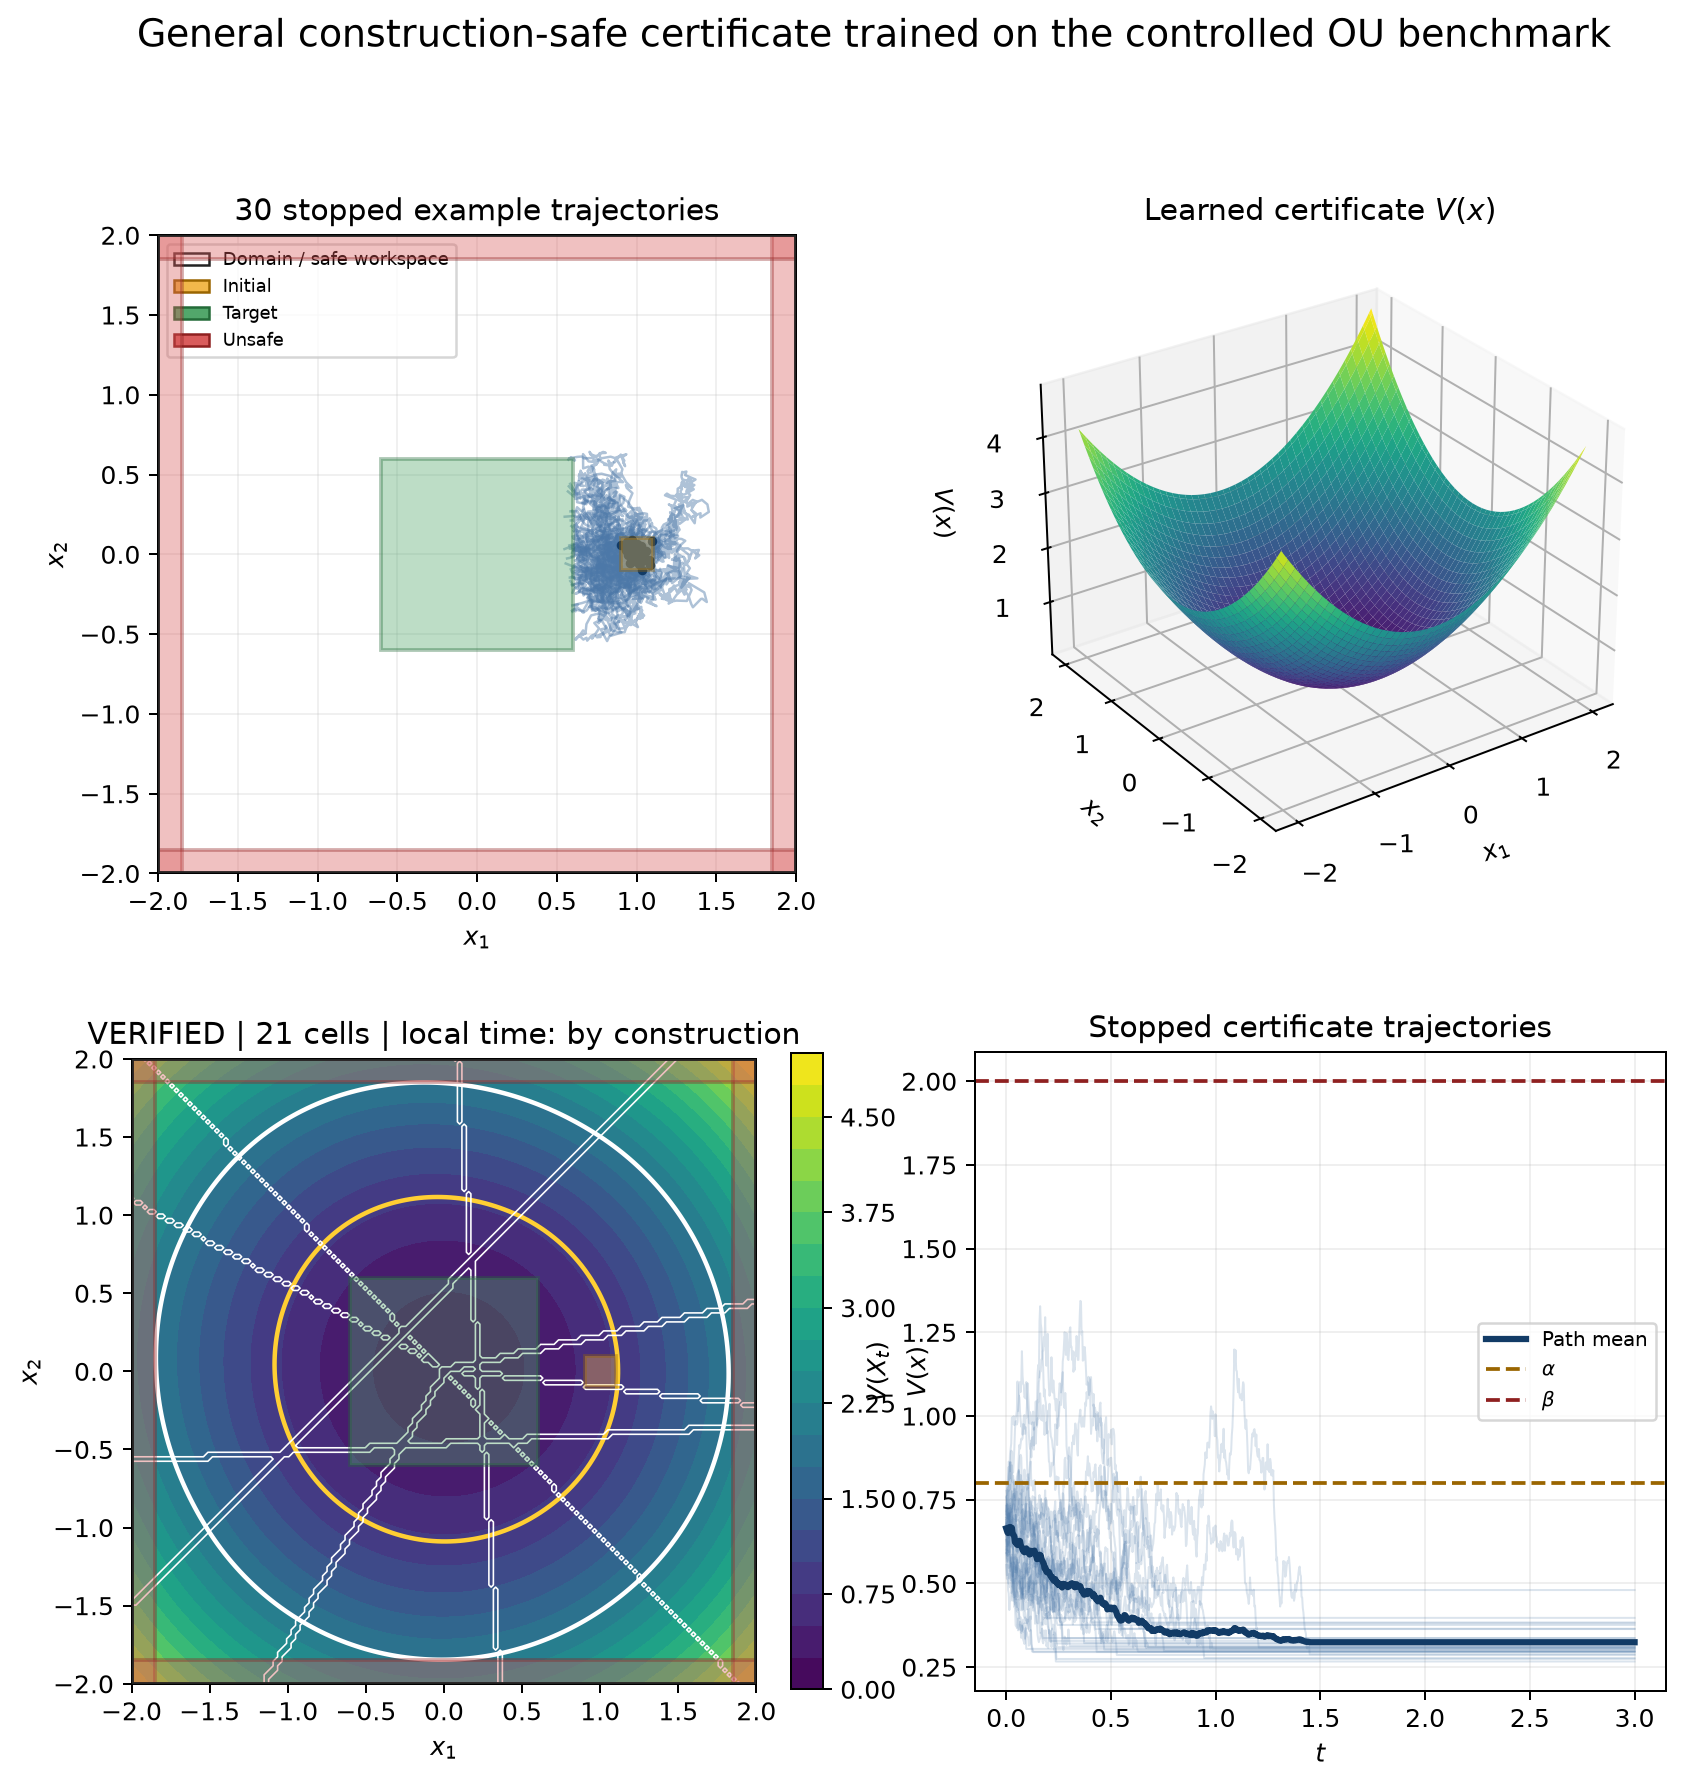
\includegraphics[width=\linewidth]{figures/verified_radial_ou_certificate.png}\par
\raggedright
{\fontsize{7.2}{8.2}\selectfont\color{Muted}
The four panels show: (1) marked reach--avoid sets and 30 stopped state
trajectories; (2) the learned surface; (3) piecewise boundaries and 21 verified
cells; and (4) the stopped processes $V(X_{t\wedge\tau})$. Simulations are
diagnostic only.\par}

\begin{bluebox}
\statusdot{Good}\hspace{1mm}\textbf{Exactly verified.}
The trained certificate has \textbf{21 PWQ cells}; all \textbf{4 max-affine
pieces} are active, and the local-time condition holds by construction. With
$\alpha=0.8$ and $\beta=2$, the certified failure-probability bound is
$\alpha/\beta=0.4$.
\end{bluebox}

\postersubsection{Training recipe}
\tinylabel{ADAM, LR $2\times10^{-3}$, BATCH 256, SEED 2026}
{\fontsize{7.8}{8.9}\selectfont
\begin{align*}
\ell_0&=\max_{X_0}[V-(\alpha-m)]_+,\\
\ell_u&=\max_{X_u}[(\beta+m)-V]_+,\\
\ell_{\partial K}&=\max_{\partial K\setminus X_T}[(\beta+m)-V]_+,\\
\ell_+&=\max_K[-V]_+,\\[-1mm]
\ell_{\mathcal L}&=\max_{K\setminus X_T}\min\{
[\mathcal LV+\varepsilon+m_{\mathcal L}]_+,[(\beta+m)-V]_+\}.
\end{align*}
$\ell=80(\ell_0+\ell_u+\ell_{\partial K}+\ell_{\mathcal L})+20\ell_+$ plus
regularisation. Verifier counterexamples are added every 25 epochs; checkpoint
200 verifies exactly. No concavity loss is needed.}
\end{minipage}

\vspace{1.5mm}
\textcolor{Rule}{\rule{\linewidth}{0.6pt}}\par
{\fontsize{7.3}{8.2}\selectfont\color{Muted}
[1] G. Neustroev et al., ``Neural Continuous-Time Supermartingale Certificates,'' AAAI 2025.
\hfill Contact: filip.morawiec@gmail.com\quad $\cdot$ \quad
Middle-of-programme result; broader architectural comparisons remain in progress.}
\end{minipage}
\end{adjustbox}
\end{document}
